In this chapter, we study a few \textbf{classic theoretical models} of accretion in isotropic media. The formal regime of these models is accretion where \textbf{angular momentum plays a minimal role} - allowing accretion to occur without the formation of a disk.
\par
In practice, this sort of accretion cannot happen: angular momentum is never really negligible. Nonetheless, it is a very simple toy model which can be used in various scenarios as long as one is careful to never trust it as a ground truth model.

\section{Bondi Accretion}

In the \textbf{Bondi Accretion} scenario, we imagine an accretor with mass $M$ embedded in an \textbf{isotropic and homogeneous} medium with density $\rho(\infty)$ and corresponding ambient sound speed $c_s(\infty)$. We assume that

\begin{enumerate}
    \item The system is \textbf{spherically symmetric},
    \item That the system accretes in a \textbf{steady state},
    \item That the flow is \textbf{inviscid, non-magnetic, and non-relativistic},
    \item That the flow follows a \textbf{polytropic equation of state}.
    \item That the flow does not rotate.
\end{enumerate}

With these assumptions, we can derive a rather beautiful formulation for the steady state accretion.

\subsection{The Heuristic Picture}
Before providing the formal proof of the Bondi model, we instead approach things from a heuristic standpoint.

\subsubsection{The Bondi Radius}

A quantity which will appear in the formal derivation presented below is the so-called \textbf{Bondi Radius} or \textbf{Sphere of Influence}. The idea is reasonably simple: in order gas to be \textbf{bound} to the central accretor, it must have velocities smaller than the escape velocity. At a radius $R$, the gravitational potential of the central body is
\[
\Phi = - \frac{GM}{R} \implies v_{\rm esc} = \sqrt{\frac{2GM}{R}}.
\]
Since the fluid has no bulk motions and is in local equilibrium, it cannot be moving faster than the local sound speed $c_s$. Thus, if 
\[
v_{\rm esc} \ge c_s,
\]
then the material will be bound to the accretor. This implies that
\[
\frac{2GM}{R} \ge c_s^2 \implies R \le \frac{2GM}{c_s^2}.
\]
We therefore introduce the \textbf{Bondi Radius}:
\vspace{20pt}
\begin{definition}
    \label{def:bondi_radius}
    The radius at which accreting material is bound to the central accretor in spherical accretion is the \textbf{Bondi Radius}, defined as
    \begin{equation}
        \label{eq:bondi_radius}
        R_{\rm Bondi} = \frac{2GM}{c_s^2}.
    \end{equation}
It is clear from inspection that this value depends on the ambient sound speed and on the mass of the accretor. If the surrounding material behaves as an ideal gas, then
\[
c_s^2 = \gamma \frac{P}{\rho} = \gamma \frac{kT}{m_p\mu}.
\]
As such,
\[
R_{\rm Bondi} = \frac{2GM}{\gamma kT} m_p\mu
\]
\end{definition}
\vspace{20pt}
It is worth looking at scalings for a few environments where Bondi accretion might be relevant. For a \textbf{stellar mass BH} in the \textbf{ISM}, with $T \sim 10^{4}\;{\rm K}$ and $c_s\sim 10\;{\rm km\;s^{-1}}$, we have
\[
R_{\rm Bondi} \sim 18 \left(\frac{M}{M_\odot}\right) \left(\frac{c_s}{10\;{\rm km\;s^{-1}}}\right)^{-2} \;{\rm AU}.
\]
\subsubsection{The Bondi Accretion Rate}

Given an ambient medium of density $\rho$ and sound speed $c_s$, gas within the
\textbf{Bondi radius}
\[
R_{\rm B} \equiv \frac{2GM}{c_s^2}
\]
is gravitationally bound to the accretor. A back-of-the-envelope estimate of the mass inflow across a sphere of radius $R_{\rm B}$ is the inward mass flux times the area:
\[
\dot M \sim ( \text{inward mass flux at } R_{\rm B}) \times 4\pi R_{\rm B}^2.
\]
For a nearly isotropic, subsonic medium, \textbf{only a fraction of the random thermal motions are directed inward at any moment}. A standard kinetic-theory estimate gives an inward flux $\simeq (\rho c_s)/4$. Using this,
\[
\dot M \sim \frac{\rho c_s}{4}\,4\pi R_{\rm B}^2
= \pi \rho c_s \left(\frac{2GM}{c_s^2}\right)^2
= 4\pi\,\frac{G^2 M^2\,\rho}{c_s^3}.
\]
This recovers the canonical scaling
\[
\boxed{\ \dot M \ \propto\ (GM)^2\,\rho\,c_s^{-3}\ }
\]
up to order-unity factors. In the next section, we'll perform the detailed derivation.

\subsection{The Detailed Bondi Model}

We have so far justified the \textbf{Bondi radius} and the \textbf{Bondi accretion rate} on heuristic grounds. Now we will go through the involved process of fully deriving and justifying the various elements of the formal derivation.

\subsubsection*{Assumptions}

In Bondi accretion, we make the following simplifying assumptions:
\vspace{0.5cm}
\begin{enumerate}
    \item \textbf{Spherical symmetry: }The entire flow is treated as spherically symmetric and the accretor is at rest relative to the ambient material. \rmk{This plays out mathematically immediately.}
    \item \textbf{Steady State}: The nature of the flow does not change over time. Formally, this means that any of the field variables $\psi$ is independent of time. \rmk{This is a trickier requirement as it allows us to define a constant accretion rate; however, we know this to be not in keeping with physical systems.}
    \item \textbf{Polytropic Equation of State}: We assume a \textit{barotropic equation of state} following the form of a polytrope
    \[
    P = \kappa \rho^\gamma.
    \]
    \rmk{In the limiting cases, we have either adiabatic flows (optically thin) or isothermal (optically thick).}
    \item \textbf{Gravity}: Is assumed to be fully Newtonian and the accretor is treated as a point mass.
    \item \textbf{No Additional Forces}: The only relevant force is that of gravity. MHD effects are ignored.
\end{enumerate}

\subsubsection*{Derivation}

Formally, we have 3 equations: the \textbf{continuity equation}, the \textbf{Euler equation}, and the \textbf{equation of state}. In this scenario, continuity provides that
\[
\underbrace{\frac{\partial \rho}{\partial t}}_{\text{$=0$ (assumpt. 2)}} + \nabla \cdot(\rho{\bf u}) = 0 \implies \frac{1}{r^2} \partial_r[r^2 \rho {\bf u}] = 0.
\]
We therefore find that
\[
r^2 \rho {\bf u} = \rm{Constant}.
\]
This is a very useful integral of the motion because the accretion rate is
\[
\dot{M} = -4\pi r^2 \rho u = {\rm Constant}.
\]
\rmk{This is deducible from the fact that we have steady flow and therefore cannot collect mass in shells.}
\par
We also have the \textbf{Euler Equation} in the form
\[
u \frac{du}{dr} + \frac{1}{\rho}\frac{dP}{dr} + \frac{GM}{r^2} = 0.
\]
Using the polytropic equation of state,
\[
\frac{dP}{dr} = \frac{dP}{d\rho} \frac{d\rho}{dr} = c_s^2 \frac{d\rho}{dr}.
\]
\rmk{Remember that $c_s^2$ is a function of radius.} From the continuity equation,
\[
\frac{1}{r^2} \partial_r (\rho r^2 u) = 0 \implies \underbrace{\rho \frac{1}{r^2}\partial(r^2u) + u \partial_r \rho}_{\text{product rule}} = 0 \implies \partial_r \log \rho = - \frac{1}{r^2 u} \partial_r ur^2,
\]
so (\rmk{substitute $\partial_r \log \rho$ and then expand out the prod. rule}),
\[
u \frac{du}{dr} - \frac{c_s^2}{ur^2} \frac{du}{dr} + \frac{GM}{r^2} = 0.
\]
If we perform some rearrangements, we find the critical equation which will consume our discussion for the rest of the section:
\begin{equation}
    \boxed{
    \frac{1}{2}\left(1-\frac{c_s^2}{u^2}\right) \frac{du^2}{dr} = -\frac{GM}{r^2} \left[1-\frac{2c_s^2 r}{GM}\right].
    }
\end{equation}

\subsubsection{The Sonic Point}
\begin{figure}
    \centering
    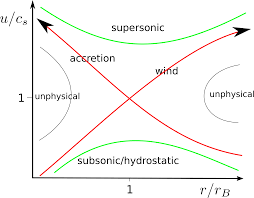
\includegraphics[width=0.75\linewidth]{Pictures/figures/bondi_regime.png}
    \caption{The parameter space of Bondi-accretion solutions. The sonic point $r_b$ is shown on the $x$-axis and the velocity on the $y$ axis.}
    \label{fig:bondi_regime}
\end{figure}
It is not immediately clear why we should have gone to all the work of building out this complicated ODE for ourselves; however, we can see that there are several very interesting features. The most important of these is that equation~\eqref{eq:bondi_critical_radius} is \textbf{singular} at 
\begin{equation}
    \label{eq:bondi_critical_radius}
    \boxed{
    r_s = \frac{GM}{2c_s^2}.
    }
\end{equation}
\rmk{Remember that $c_s$ is still a function of the radius. This means that this is \textbf{implicit}.} This is the so-called \textbf{sonic point} of the flow: \textit{if} the flow is going to make a transition to or from \textbf{sub-sonic} to \textbf{super-sonic}, it \textit{must occur at $r_s$.} This means that there are 4 important regimes to consider:
\vspace{0.5cm}
\begin{enumerate}
    \item \textbf{Transitioning Solution}: If we enforce that $u = c_s$ at the sonic radius, then the solution is entirely determined by the choice of behavior as $r\to \infty$ or by the choice of behavior as $r\to0$. If we let $u \to 0$ at $\infty$, then we obtain \textbf{accreting flows} featuring a transition point, and if we permit $u \to 0$ as $r\to 0$, then we obtain \textbf{wind flows} with transition points.
    \item \textbf{Non-Transitioning Solutions}: If a solution is not going to have $u=c_s$, then one \textit{must let $du^2/dr = 0$} at the sonic radius. In this case, the entire solution is fixed either by the behavior at either asymptote or by the behavior (the velocity) at the sonic point.
\end{enumerate}
\vspace{0.5cm}

\subsubsection{Bernoulli Flow}
We have now clarified the general behavior of the ODE we wish to solve and identified the relevant regimes. Most importantly, we are now able to recognize that uniqueness of our solution can be guaranteed by specifying the behavior both at the critical point and at $\infty$. Let us now fully solve the problem. To do so, we will apply \textbf{Bernoulli's Theorem}:
\[
u \frac{du}{dr}+ \nabla(h+\phi) = 0 \implies \frac{1}{2} u^2 + h + \phi = 0.
\]
For a \textbf{barotropic equation of state}, the specific enthalpy is
\[
h = \int \frac{dP}{\rho} = \int \frac{dP}{d\rho} \frac{1}{\rho} d\rho = \frac{K\gamma}{\gamma -1} \rho^{\gamma - 1} = \frac{c_s^2}{\gamma -1}.
\]
Thus,
\begin{equation}
    \frac{u^2}{2} + \frac{c_s^2}{\gamma -1} - \frac{GM}{r} = \rm{Constant}.
\end{equation}
\rmk{In the isothermal case, we actually need to have a logarithm here instead of $\gamma -1$.}
\par
Now, for \textbf{accreting flows}, we have $u(\infty) = 0$. Thus,
\[
c_s^2(\infty) = C(\gamma-1) \implies C = \frac{c_s^2(\infty)}{\gamma -1}.
\]
Additionally, the sonic point requires that
\[
c_s^2(r_s) = \frac{GM}{2r_s},
\]
so at $r_s$, we have
\[
\frac{c_s^2(r_s)}{2} + \frac{c_s^2(r_s)}{\gamma -1} - 2c_s^2(r_s) = \frac{c_s^2(\infty)}{\gamma -1}.
\]
So
\begin{equation}
\boxed{\
    c_s(r_s) = c_s(\infty) \left(\frac{2}{5 - 3\gamma}\right)^{1/2}
    }
\end{equation}
\rmk{NOTES: degeneracies!}
The mass accretion rate is constant at all radii, so we can evaluate it at the sonic point and find
\begin{equation}
    \boxed{
    \dot{M} = \pi G^2 M^2 \frac{\rho(\infty)}{c_s^3(\infty)} \left[\frac{2}{5-3\gamma}\right]^{(5-3\gamma)/2(\gamma-1)}.
    }
\end{equation}
\subsubsection{The Accretion Radius}

The Bondi solution motivates the introduction of a characteristic length scale, the
\textbf{accretion radius}, defined as
\begin{equation}
    \label{eq:bondi_radius}
    r_{\rm acc} \equiv \frac{2GM}{c_s^2(\infty)}.
\end{equation}
This can be understood from a simple energetic argument. At radius $r$, the
\textbf{gravitational binding energy per unit mass} is
\[
E_{\rm grav} \sim \frac{GM}{r},
\]
while the \textbf{thermal energy per unit mass} of the gas is set by the sound speed,
\[
E_{\rm th} \sim c_s^2(\infty).
\]
The radius $r_{\rm acc}$ is defined as the point where these two energy scales balance:
inside this radius, gravitational attraction dominates over thermal motions, so gas is
gravitationally captured by the accretor. Outside this radius, pressure forces can
support the gas against collapse. Thus, $r_{\rm acc}$ plays the role of an effective
``sphere of influence'' for accretion.

\begin{remark}
Note that $r_{\rm acc}$ is distinct from the precise sonic radius $r_s$, which depends
on the local sound speed $c_s(r_s)$. The accretion radius is defined in terms of the
\emph{asymptotic} sound speed at infinity, and provides a more intuitive, order-of-magnitude
measure of the capture region.
\end{remark}

\subsubsection{Free-Fall Behavior Beyond the Sonic Point}

Once the gas passes through the sonic point, the flow is \textbf{supersonic}. In this
regime, pressure forces are negligible compared to inertia and gravity: the gas
effectively undergoes free fall. This allows us to extract the asymptotic scaling of
velocity, density, and temperature in the inner region.

\paragraph{Velocity:} In free fall onto a point mass, the velocity is set by the
gravitational potential:
\[
u(r) \sim \left(\frac{2GM}{r}\right)^{1/2}.
\]

\paragraph{Density:} The accretion rate is constant at all radii,
\[
\dot{M} = 4\pi r^2 \rho u.
\]
Substituting the free-fall velocity,
\[
\rho(r) \sim \frac{\dot{M}}{4\pi r^2 u(r)} \;\propto\; r^{-3/2}.
\]

\paragraph{Temperature:} For a polytropic gas,
\[
T \propto \frac{P}{\rho} \propto \rho^{\gamma-1}.
\]
Thus, in the inner free-fall region,
\[
T(r) \;\propto\; r^{-3(\gamma-1)/2}.
\]
For example:
\begin{itemize}
    \item Isothermal case ($\gamma=1$): $T(r) = \rm{const}$.  
    \item Adiabatic monoatomic gas ($\gamma=5/3$): $T(r) \propto r^{-1}$.
\end{itemize}

\subsection{Feasibility as an Accretion Mechanism}

A natural question is whether Bondi accretion can power luminous sources such as
X-ray binaries (XRBs), ultraluminous X-ray sources (ULXs), or active galactic nuclei (AGN).
From the steady, spherical solution one finds
\begin{equation}
\dot M_{\rm B} \;=\; 4\pi\,\lambda(\gamma)\,\frac{(GM)^2\,\rho_\infty}{c_{s,\infty}^{\,3}}
\qquad\Rightarrow\qquad
L_{\rm B} \;\equiv\; \eta\,\dot M_{\rm B} c^2
\,=\, 4\pi\,\lambda(\gamma)\,\eta\,\frac{G^2 M^2 \rho_\infty c^2}{c_{s,\infty}^{\,3}},
\label{eq:bondi_luminosity}
\end{equation}
where $\lambda(\gamma)\!\sim\!{\cal O}(0.1\!\!-\!\!1)$ depends weakly on the equation of state,
$\eta$ is a (model-dependent) radiative efficiency, and $\rho_\infty=\mu m_p n$.
For back-of-the-envelope estimates it is common to set $\lambda(\gamma)\simeq 1$.

\paragraph{Numerical scalings.}
Adopting $\mu\simeq 1.3$ and normalizing to $n=1~{\rm cm^{-3}}$ and $c_s=10~{\rm km\,s^{-1}}$,
\begin{align}
\dot M_{\rm B} &\;\simeq\; 4.8\times 10^{11}\,
\left(\frac{n}{1~{\rm cm^{-3}}}\right)
\left(\frac{\mu}{1.3}\right)
\left(\frac{M}{M_\odot}\right)^{\!2}
\left(\frac{c_s}{10~{\rm km\,s^{-1}}}\right)^{-3}
\ {\rm g\,s^{-1}},\\[3pt]
L_{\rm B} &\;\simeq\; 4.3\times 10^{31}\,
\left(\frac{\eta}{0.1}\right)
\left(\frac{n}{1~{\rm cm^{-3}}}\right)
\left(\frac{\mu}{1.3}\right)
\left(\frac{M}{M_\odot}\right)^{\!2}
\left(\frac{c_s}{10~{\rm km\,s^{-1}}}\right)^{-3}
\ {\rm erg\,s^{-1}}.
\label{eq:bondi_numeric}
\end{align}
These make explicit the key dependencies: $L_{\rm B}\propto M^2\,n\,c_s^{-3}$.

\paragraph{Comparison to Eddington.}
The Eddington luminosity is
\begin{equation}
L_{\rm Edd} \;\simeq\; 1.26\times 10^{38}\left(\frac{M}{M_\odot}\right)\ {\rm erg\,s^{-1}}.
\end{equation}
Hence
\begin{equation}
\frac{L_{\rm B}}{L_{\rm Edd}}
\;\simeq\;
3.4\times 10^{-7}\,
\left(\frac{\eta}{0.1}\right)
\left(\frac{n}{1~{\rm cm^{-3}}}\right)
\left(\frac{\mu}{1.3}\right)
\left(\frac{M}{10\,M_\odot}\right)
\left(\frac{c_s}{10~{\rm km\,s^{-1}}}\right)^{-3}.
\end{equation}

\paragraph{Concrete cases.}
\begin{itemize}
\item \textbf{Stellar-mass accretor in the warm ISM} ($M=10\,M_\odot$, $n\simeq 1~{\rm cm^{-3}}$, $c_s\simeq 10~{\rm km\,s^{-1}}$):\\
$L_{\rm B}\sim 4\times 10^{33}\,{\rm erg\,s^{-1}} \ll 10^{36\!-\!39}\,{\rm erg\,s^{-1}}$ (typical XRB/ULX).
Thus, \emph{Bondi accretion from the diffuse ISM is orders of magnitude too feeble}
to power luminous XRBs/ULXs.

\item \textbf{Wind-fed HMXB (Bondi–Hoyle capture).} The relevant speed is the \emph{relative wind speed}
($v_{\rm rel}\!\gg\! c_s$), so take $c_s\!\to\! v_{\rm eff}\simeq v_{\rm rel}$. With $v_{\rm rel}\sim 1500~{\rm km\,s^{-1}}$ and $M=10\,M_\odot$,
$L_{\rm B}$ is suppressed by $(1500/10)^{-3}\!\sim\!3\times 10^{-6}$ relative to the ISM case, i.e.\ $L_{\rm B}\sim 10^{27}\,{\rm erg\,s^{-1}}$.
\emph{Wind speed crushes the capture radius and luminosity}; luminous HMXBs require Roche-lobe overflow or much denser/slower inflow.

\item \textbf{SMBH in galactic gas.}
For $M=10^{6}\,M_\odot$ and \emph{cool/warm} gas ($n\!\sim\!1~{\rm cm^{-3}}$, $c_s\!\sim\!10~{\rm km\,s^{-1}}$),
Eq.~\eqref{eq:bondi_numeric} gives $L_{\rm B}\sim 4\times 10^{43}\,{\rm erg\,s^{-1}}$, comparable to $L_{\rm Edd}\!\sim\!1\times 10^{44}\,{\rm erg\,s^{-1}}$.
However, realistic circumnuclear media are often \emph{hot and tenuous} ($n\!\sim\!0.1~{\rm cm^{-3}}$, $c_s\!\sim\!400~{\rm km\,s^{-1}}$),
which suppresses $L_{\rm B}$ by $\sim (0.1)\times (400/10)^{-3}\!\approx\!1.6\times 10^{-3}$,
yielding $L_{\rm B}\sim 7\times 10^{37}\,{\rm erg\,s^{-1}} \ll L_{\rm Edd}$.
\end{itemize}
\subsection*{Summary and Key Formulae}

Bondi accretion provides the simplest classical model for spherically symmetric accretion onto a compact object. While highly idealized, it illustrates several key physical principles:

\begin{itemize}
    \item The flow is uniquely determined by the requirement that it pass smoothly through the \textbf{sonic point}. This makes the solution transonic, subsonic at infinity and supersonic near the accretor. 
    \item The \textbf{accretion radius} 
    \[
    r_{\rm acc} = \frac{2GM}{c_s^2(\infty)}
    \]
    defines the natural scale inside which gravity dominates over thermal pressure. Gas at $r \lesssim r_{\rm acc}$ is gravitationally captured.
    \item The \textbf{Bondi accretion rate} can be expressed either in terms of $r_{\rm acc}$ or directly in terms of asymptotic conditions:
    \[
    \dot{M}_{\rm Bondi} \;\sim\; \pi r_{\rm acc}^2 \rho_\infty c_s(\infty),
    \qquad
    \dot{M}_{\rm Bondi} = \pi G^2 M^2 \frac{\rho(\infty)}{c_s(\infty)^3}\left[\frac{2}{5-3\gamma}\right]^{(5-3\gamma)/2(\gamma-1)}.
    \]
    The exact prefactor depends on the adiabatic index $\gamma$, but the scaling is robust.
    \item Inside the sonic point, the flow is effectively in free fall, with the following power-law scalings:
    \[
    u(r) \propto r^{-1/2}, \qquad \rho(r) \propto r^{-3/2}, \qquad T(r) \propto r^{-3(\gamma-1)/2}.
    \]
    For an adiabatic monoatomic gas ($\gamma=5/3$), this gives $T(r) \propto r^{-1}$.
    \item Order-of-magnitude estimates show that for compact objects, the rates are very small compared to what is observable:
    \[
    \dot{M}_{\rm Bondi} \sim 1.4 \times 10^{11}\;\; \left(\frac{M}{M_\odot}\right)^2 \left(\frac{\rho_\infty}{1\,{\rm cm}^{-3}\;m_p}\right)\left(\frac{10\,{\rm km/s}}{c_s(\infty)}\right)^3 \;{\rm g\,s^{-1}}.
    \]
    For example:
    \begin{itemize}
        \item White Dwarf ($M \sim 1M_\odot$, $R \sim 10^9\,$cm): $\dot{M} \sim 10^{12}\,{\rm g\,s^{-1}}$.
        \item Neutron Star ($M \sim 1.4M_\odot$, $R \sim 10^6\,$cm): $\dot{M} \sim 10^{13}\,{\rm g\,s^{-1}}$.
    \end{itemize}
    
Even though compact objects have deep gravitational potentials, the sparse interstellar medium is simply too dilute: Bondi accretion in realistic astrophysical settings is far below detectable levels.
\end{itemize}
\vspace{0.5cm}

\begin{bigidea}
\textbf{Bondi Accretion: Must-Remember Formulae}
\begin{align*}
r_{\rm acc} &= \frac{2GM}{c_s^2(\infty)} \\[6pt]
\dot{M}_{\rm Bondi} &\sim \pi r_{\rm acc}^2 \rho_\infty c_s(\infty) \;\;\;\; \propto \frac{(GM)^2 \rho_\infty}{c_s^3(\infty)} \\[6pt]
\rho(r) &\propto r^{-3/2}, \qquad T(r) \propto r^{-3(\gamma-1)/2}, \qquad u(r) \propto r^{-1/2} \\[6pt]
\dot{M}_{\rm WD} &\sim 10^{12} \;\left(\frac{M}{M_\odot}\right)^2\;{\rm g\,s^{-1}}, \qquad
\dot{M}_{\rm NS} \sim 10^{13} \;\left(\frac{M}{M_\odot}\right)^2\;{\rm g\,s^{-1}}
\end{align*}
\textbf{Takeaway:} Bondi accretion sets the baseline scale for spherical capture from a uniform medium, but the resulting accretion rates are far too small to be astrophysically significant in most environments.
\end{bigidea}

\begin{conceptbox}

Practical applications include:
\begin{itemize}
    \item Isolated neutron stars or black holes accreting from the interstellar medium.
    \item Quiescent supermassive black holes (e.g.\ Sgr A*) accreting from hot gas in galaxies.
    \item Wind-fed X-ray binaries, modeled with the related Bondi--Hoyle--Lyttleton formalism.
    \item Central black holes in galaxy clusters accreting from the intracluster medium.
    \item Subgrid prescriptions for black hole growth in cosmological simulations.
\end{itemize}
In each case, the Bondi rate provides an order-of-magnitude estimate of fuel availability, 
though real systems are often modified by angular momentum, turbulence, or feedback processes.
\end{conceptbox}

\section{Bondi--Hoyle--Lyttleton Accretion}
\label{sec:BHL}

When the accretor moves with respect to the ambient medium (or, equivalently, the medium flows past the accretor), spherical symmetry is broken and the appropriate idealized model is \textbf{Bondi--Hoyle--Lyttleton (BHL)} accretion. This captures \emph{gravitational focusing} of upstream streamlines into a downstream \emph{accretion column} and is the canonical toy model for wind-fed accretion in high-mass X-ray binaries, compact objects moving through the ISM, and black holes traversing gaseous environments.
\par
We consider an accretor of mass $M$ immersed in a uniform medium with density $\rho_\infty$ and sound speed $c_{s,\infty}$, experiencing a uniform relative flow with speed $v_{\rm rel}$ (equivalently, the accretor moves at $v_{\rm rel}$
through a static medium). We assume:
\vspace{10pt}
\begin{enumerate}
    \item \textbf{Steady state in the accretor frame}.
    \item \textbf{Inviscid, non-magnetic, non-relativistic} hydrodynamics.
    \item A \textbf{barotropic/polytropic} equation of state, $P=K\rho^\gamma$.
    \item \textbf{Point-mass gravity} for the accretor.
    \item The upstream medium is \textbf{homogeneous and isotropic} at infinity.
\end{enumerate}
\vspace{10pt}

\subsection{The Heuristic Picture}

In the accretor frame, upstream gas with impact parameter $b$ is focused by gravity. Particles with sufficiently small $b$ are gravitationally captured and funneled into a downstream \emph{wake} that feeds the accretor. Balancing kinetic/thermal energy against gravitational binding suggests the characteristic \textbf{accretion radius}
\begin{equation}
    r_{\rm acc} \;\equiv\; \frac{2GM}{v_{\rm eff}^2},
    \qquad
    v_{\rm eff} \;\equiv\; \sqrt{v_{\rm rel}^2 + c_{s,\infty}^2},
    \label{eq:bhl_racc}
\end{equation}
which reduces to the Bondi radius when $v_{\rm rel}\to 0$. Streamlines with $b\lesssim r_{\rm acc}$ are strongly focused and can be captured. A geometric capture argument gives a mass flux through the ``accretion cylinder''
of area $\pi r_{\rm acc}^2$:
\[
\dot M \sim \pi r_{\rm acc}^2 \rho_\infty v_{\rm eff}
= \pi \left(\frac{2GM}{v_{\rm eff}^2}\right)^2 \rho_\infty v_{\rm eff}
= 4\pi \frac{G^2 M^2 \rho_\infty}{v_{\rm eff}^{\,3}}.
\]
A more careful hydrodynamic analysis (and numerical calibration) yields the standard \textbf{BHL accretion rate}
\begin{equation}
    \boxed{
    \dot M_{\rm BHL} \;=\; 4\pi\,\lambda(\gamma,{\cal M})\,
    \frac{G^2 M^2\,\rho_\infty}{\big(v_{\rm rel}^2 + c_{s,\infty}^2\big)^{3/2}}
    }
    \label{eq:bhl_rate}
\end{equation}
where ${\cal M}\equiv v_{\rm rel}/c_{s,\infty}$ is the upstream Mach number and $\lambda(\gamma,{\cal M})$ is an order-unity dimensionless coefficient (reducing to the Bondi $\lambda(\gamma)$ for ${\cal M}\to 0$). The \emph{key scaling} is robust:
\[
\dot M_{\rm BHL} \;\propto\; M^2\,\rho_\infty\,v_{\rm eff}^{-3}.
\]
Thus, BHL accretion is \emph{extremely sensitive} to the relative speed $v_{\rm rel}$ and the upstream temperature through $c_{s,\infty}$.

\subsection{BHL Accretion Morphology}

The qualitative flow depends on the \textbf{Mach number} ${\cal M}$:

\paragraph{Subsonic (${\cal M}<1$):}
The pattern resembles a gently deflected flow with broad focusing into the wake.
Pressure communicates upstream, smoothing gradients.

\paragraph{Supersonic (${\cal M}>1$):}
A \textbf{bow shock} forms upstream of the accretor with a stand-off distance
$R_{\rm sh}\sim {\cal O}(r_{\rm acc})$. Downstream, a narrow, dense \emph{accretion column} forms along the symmetry axis and terminates at the inner boundary. The global topology is approximately axisymmetric but can exhibit
time-dependent structure depending on cooling and dimensionality.

\subsubsection{Dynamical Drag (Gaseous Dynamical Friction)}

Gravitational focusing produces an overdense wake that exerts a \emph{drag} on the
accretor. To leading order one expects a drag of order the accretion \emph{momentum}
flux, $F_{\rm drag}\sim \dot M_{\rm BHL}\,v_{\rm rel}$, with additional
contributions from the extended wake (``dynamical friction''). The drag scales
$\propto \rho_\infty M^2 v_{\rm eff}^{-2}$ and can be dynamically important for
compact objects in dense media or for SMBHs moving in galactic gas.

\subsubsection{Angular Momentum and Disc Formation}

Even tiny upstream gradients (in density or velocity) or turbulence impart specific
angular momentum to the captured flow. Although the \emph{ideal} BHL solution is
axisymmetric with zero net $j$, realistic BHL flows generically form small discs or
\emph{mini-discs} around the accretor once material circularizes at $r_{\rm circ}\!\sim\! j^2/(GM)$. Thus, BHL is best viewed as the \emph{capture} stage; the inner accretion geometry often departs from the purely ballistic picture.

\subsection{Feasibility and Order-of-Magnitude Estimates}

Using Eq.~\eqref{eq:bhl_rate}, a handy normalization is
\begin{equation}
\dot M_{\rm BHL} \;\simeq\;
4\pi\,\lambda\,\frac{G^2 M^2 \rho_\infty}{\big(v_{\rm rel}^2 + c_{s,\infty}^2\big)^{3/2}}
\;\approx\;
6.3\times 10^{15}\,\lambda\,
\left(\frac{M}{10\,M_\odot}\right)^{\!2}
\left(\frac{n}{10^{10}\,{\rm cm^{-3}}}\right)
\left(\frac{v_{\rm eff}}{1000\,{\rm km\,s^{-1}}}\right)^{-3}
\ \frac{{\rm g}}{\rm s},
\end{equation}
where $\rho_\infty=\mu m_p n$ and $v_{\rm eff}=\sqrt{v_{\rm rel}^2+c_{s,\infty}^2}$.
The $v_{\rm eff}^{-3}$ dependence means fast winds \textbf{dramatically quench accretion}, while dense, slow flows can yield appreciable $\dot M$. A corresponding luminosity estimate $L\simeq \eta \dot M c^2$ must be tempered by geometry (mini-discs, shocks) and radiative efficiency (often $\eta\ll 0.1$ for inefficient, quasi-spherical flows).

\subsection*{Summary and Key Formulae}

\begin{bigidea}
\textbf{Bondi--Hoyle--Lyttleton: Must-Remember Formulae}
\begin{align*}
r_{\rm acc} &= \frac{2GM}{v_{\rm rel}^2 + c_{s,\infty}^2},
\qquad
v_{\rm eff}=\sqrt{v_{\rm rel}^2+c_{s,\infty}^2} \\[6pt]
\dot M_{\rm BHL} &= 4\pi\,\lambda(\gamma,{\cal M})\,
\frac{G^2 M^2 \rho_\infty}{\big(v_{\rm rel}^2 + c_{s,\infty}^2\big)^{3/2}}
\;\;\;\; \propto\; M^2 \rho_\infty v_{\rm eff}^{-3} \\[6pt]
\text{Bow shock (}\mathcal{M}>1\text{)}&:\ \ R_{\rm sh}\sim \mathcal{O}(r_{\rm acc}),\ \ \text{narrow downstream column} \\[6pt]
F_{\rm drag} &\sim \dot M_{\rm BHL}\,v_{\rm rel}\ \ \propto\ \rho_\infty M^2 v_{\rm eff}^{-2}
\end{align*}
\textbf{Takeaway:} BHL accretion is a gravitational capture process regulated by
$v_{\rm eff}^{-3}$. It smoothly connects to Bondi for $v_{\rm rel}\!\to\!0$, but in
wind-fed systems the large $v_{\rm rel}$ (and often large $c_{s,\infty}$) suppresses
$\dot M$ unless the flow is sufficiently dense and slow. Small angular-momentum
seeds generically produce mini-discs, making BHL a capture model rather than a
strictly disc-free accretion solution.
\end{bigidea}

